\section{Experiments}

\begin{frame}
	\frametitle{Experimental Evaluation}
	
	\Large
	
	\vspace{0.3cm}
	
	\begin{enumerate}
		\item Simulating 3 moving Aldebaran Nao robots tracking the ball movements on the field
		
		\seti
	\end{enumerate}
	
	\begin{figure}
		\centering
		
		\begin{tikzpicture}
			\node at (0,0) [draw=white,ultra thick,inner sep=0pt]
			{
				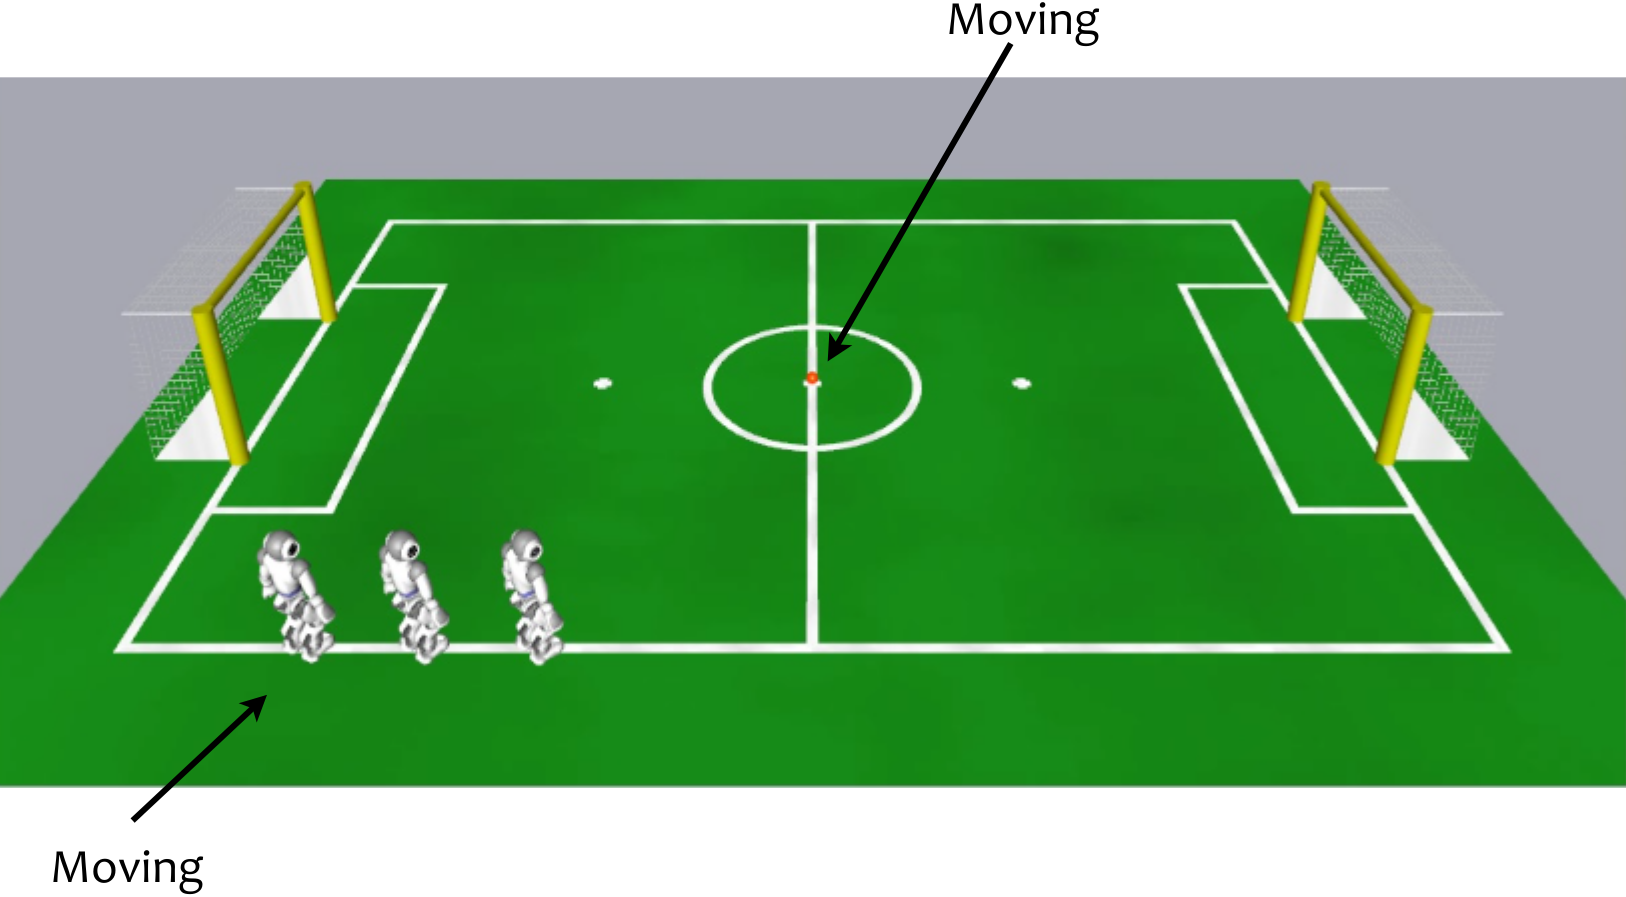
\includegraphics[width=0.82\linewidth]{Figures/Scenario-1}
			};
		\end{tikzpicture}
	\end{figure}
\end{frame}

\begin{frame}
	\frametitle{Experimental Evaluation}
	\framesubtitle{Tracking Results}
	
	\vspace{-1cm}
	
	\begin{figure}
		\centering
		
		\begin{tikzpicture}
			\node at (0,0) [draw=white,ultra thick,inner sep=0pt]
			{
				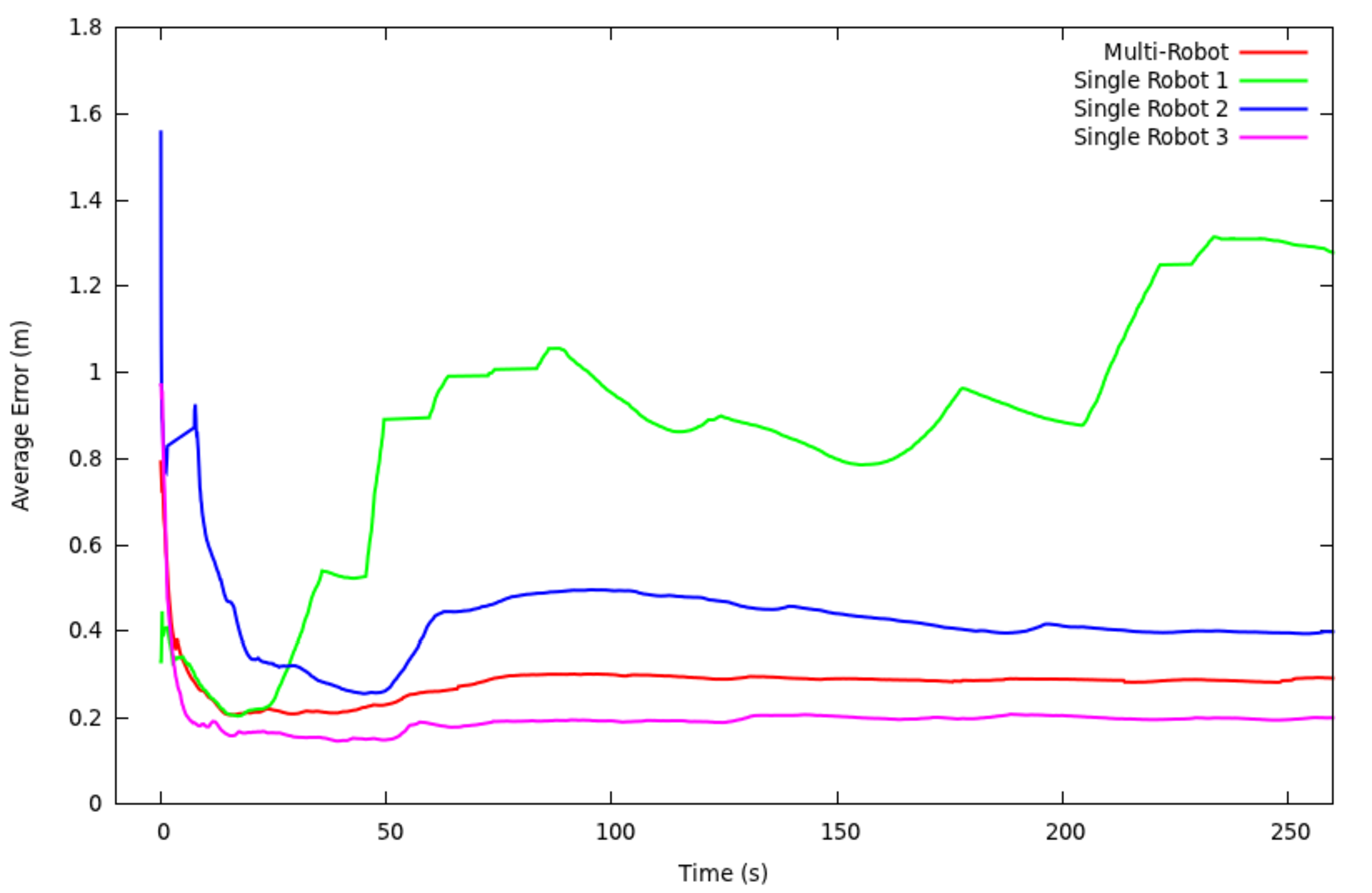
\includegraphics[width=0.85\linewidth]{Figures/Result-Scenario-1}
			};
		\end{tikzpicture}
	\end{figure}
	
	\vspace{-4cm}
	
	\begin{tabbing}
		\scriptsize
		\hspace{3.83cm}
		
		\textbf{Multi-Robot estimation follows the best single ones}
	\end{tabbing}
	
	\vspace{-0.85cm}
	
	\begin{tabbing}
		\Huge
		\hspace{8cm}
		$ \searrow $
	\end{tabbing}
\end{frame}

\begin{frame}
	\frametitle{Experimental Evaluation}
	\framesubtitle{Tracking Robustness}
	
	\vspace{-1.515cm}
	
	\begin{figure}
		\centering
		
		\begin{tikzpicture}
			\node at (0,0) [draw=white,ultra thick,inner sep=0pt]
			{
				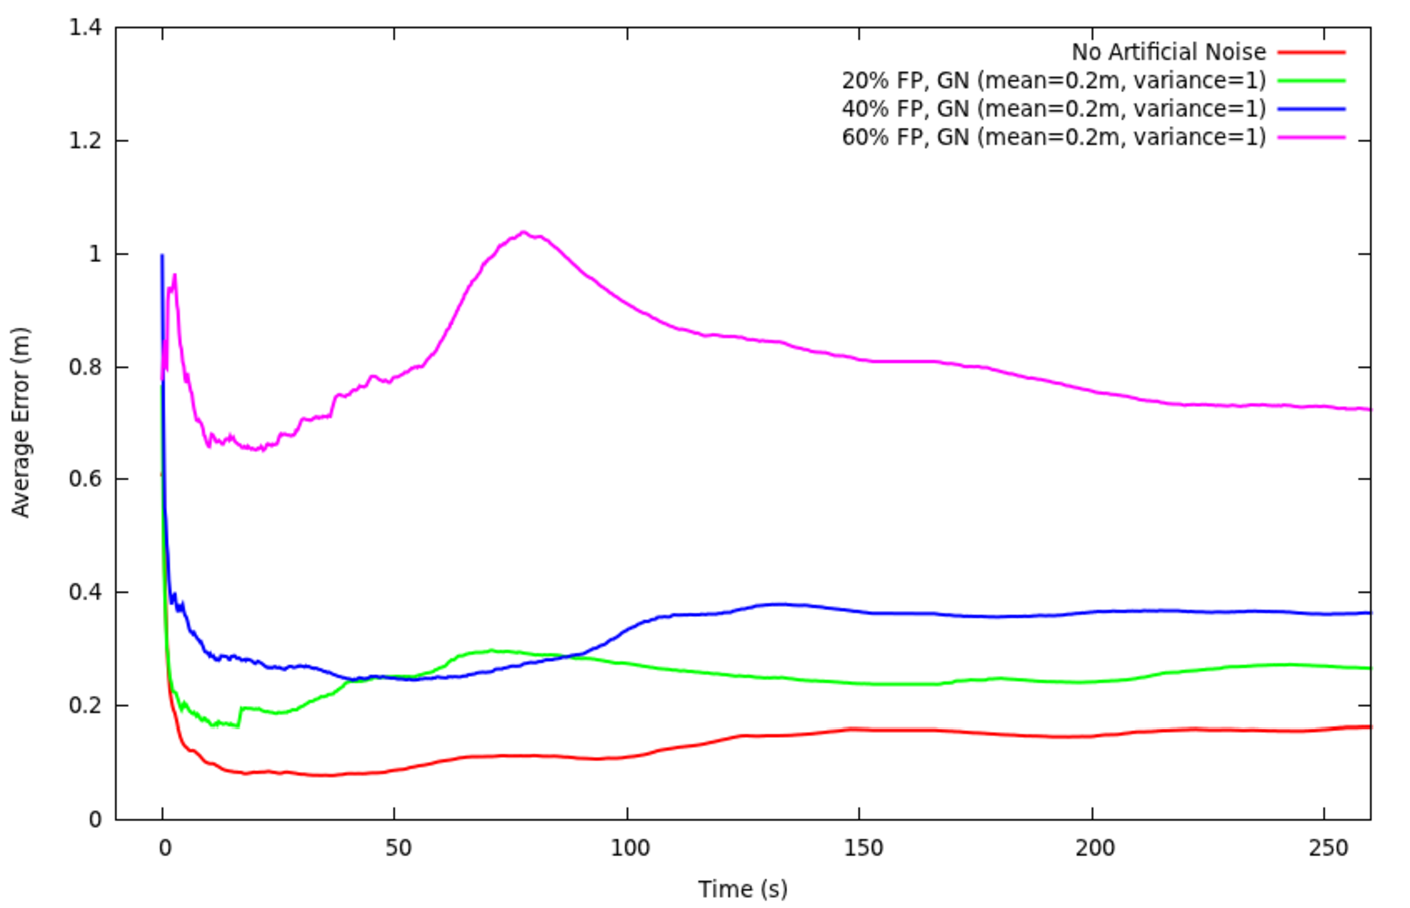
\includegraphics[width=0.85\linewidth]{Figures/Robustness-Scenario-1}
			};
		\end{tikzpicture}
	\end{figure}
	
	\vspace{-4cm}
	
	\begin{tabbing}
		\scriptsize
		\hspace{3.83cm}
		
		\textbf{Robustness up to 40\% of false positives}
	\end{tabbing}
\end{frame}

\begin{frame}
	\frametitle{Experimental Evaluation}
	
	\Large
	
	\vspace{-0.94cm}
	
	\begin{enumerate}
		\conti
		
		\item Simulating 3 Aldebaran Nao robots playing soccer, alternatively forced to be
			  inversely localized
		
		\seti
	\end{enumerate}
	
	\vspace{-0.8cm}
	
	\begin{columns}[T]
		\column{1.02\textwidth}
		
	\begin{figure}
		\centering
		
		\begin{tikzpicture}
			\node at (0,0) [draw=white,ultra thick,inner sep=0pt]
			{
				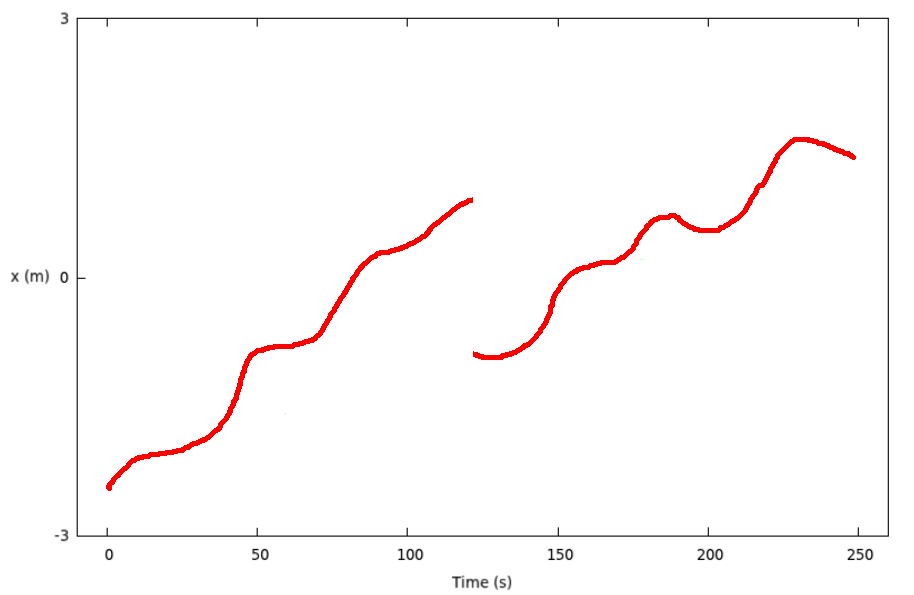
\includegraphics[width=0.34\linewidth]{Figures/Result-Scenario-2_Robot-1}
			};
			\node at (4.1,0) [draw=white,ultra thick,inner sep=0pt]
			{
				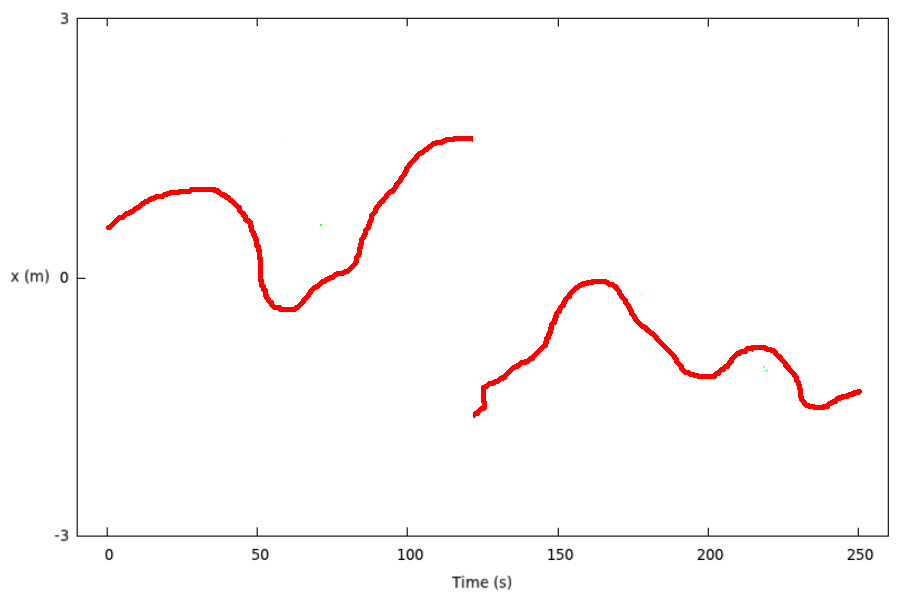
\includegraphics[width=0.34\linewidth]{Figures/Result-Scenario-2_Robot-2}
			};
			\node at (0,-2.9) [draw=white,ultra thick,inner sep=0pt]
			{
				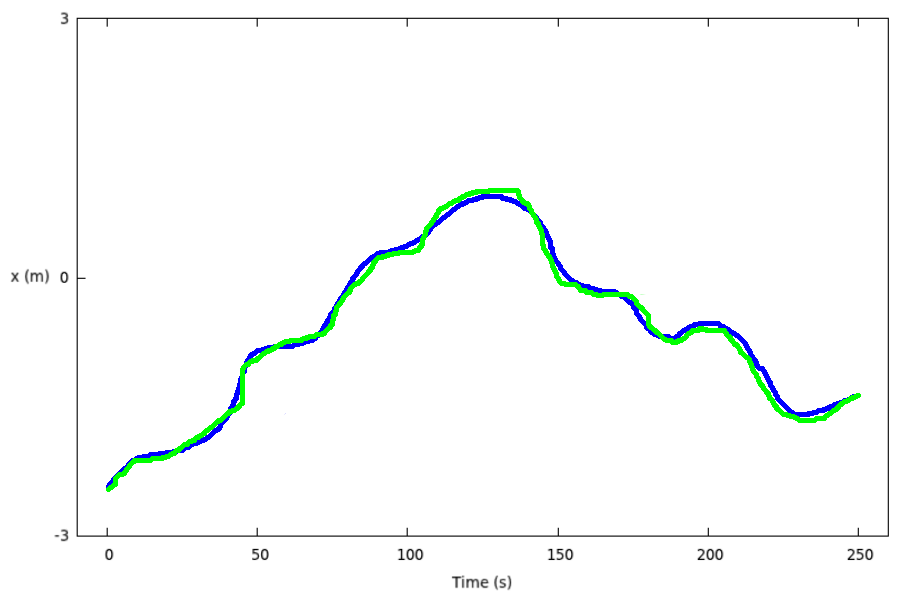
\includegraphics[width=0.34\linewidth]{Figures/Result-Scenario-2_Robot-1-GT}
			};
			\node at (4.1,-2.9) [draw=white,ultra thick,inner sep=0pt]
			{
				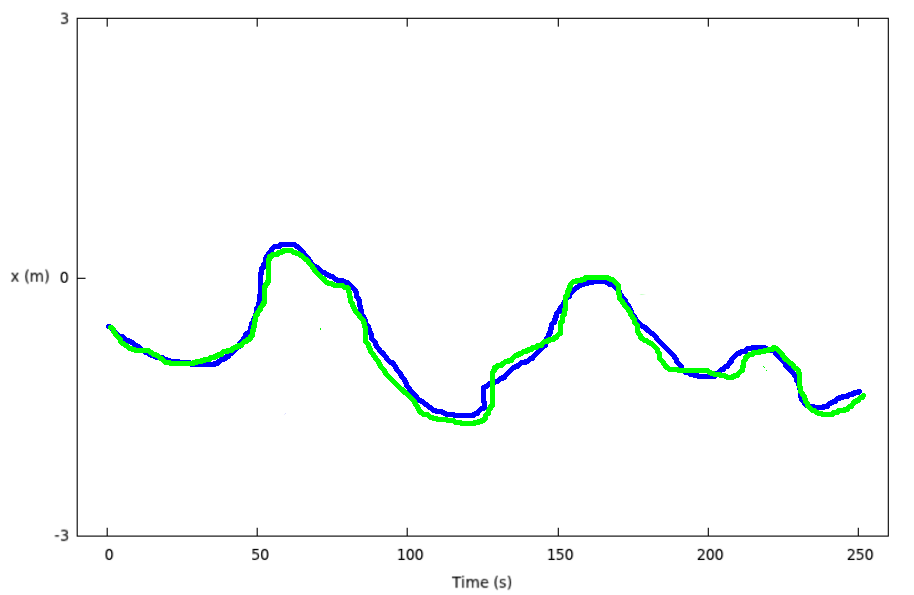
\includegraphics[width=0.34\linewidth]{Figures/Result-Scenario-2_Robot-2-GT}
			};
			\node at (8.2,0) [draw=white,ultra thick,inner sep=0pt]
			{
				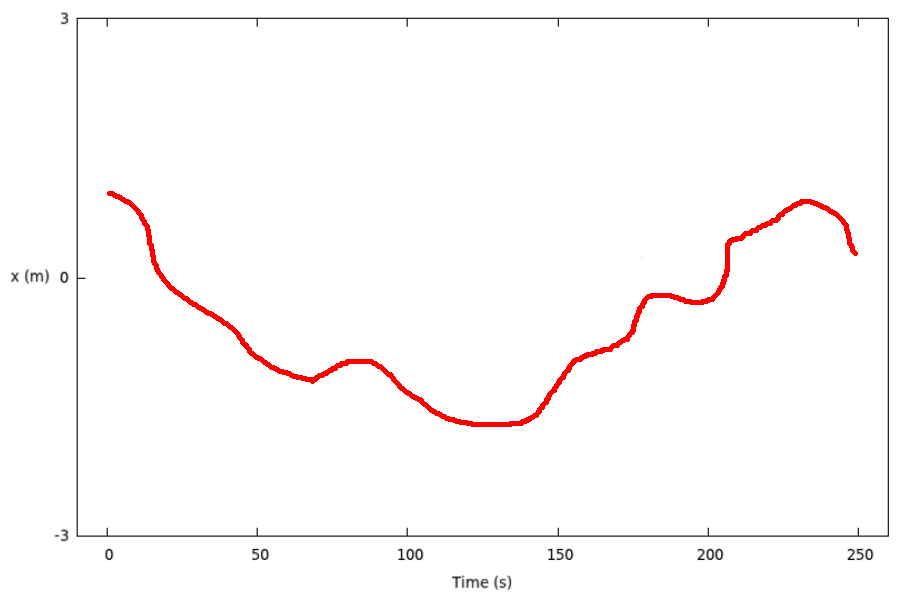
\includegraphics[width=0.34\linewidth]{Figures/Result-Scenario-2_Robot-3}
			};
			\node at (8.2,-2.9) [draw=white,ultra thick,inner sep=0pt]
			{
				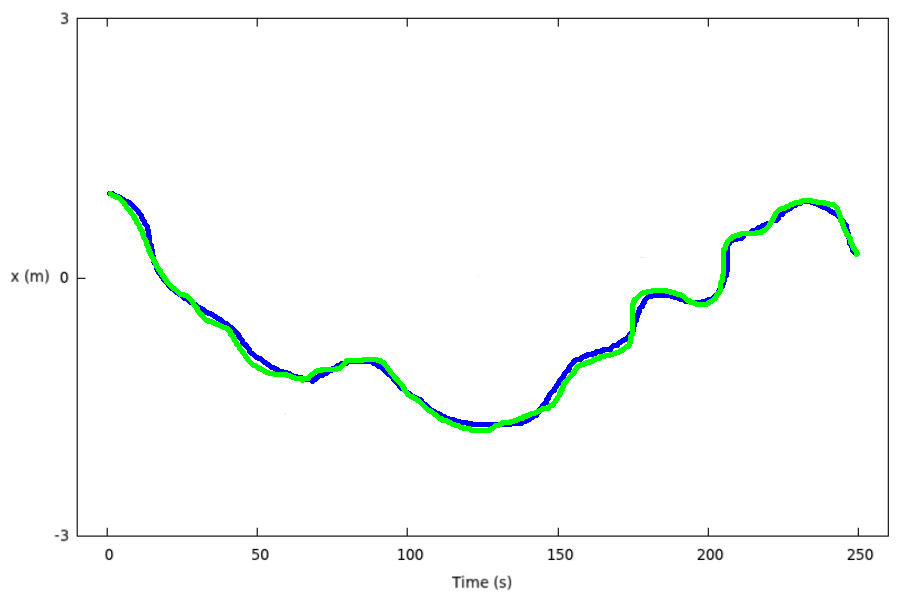
\includegraphics[width=0.34\linewidth]{Figures/Result-Scenario-2_Robot-3-GT}
			};
		\end{tikzpicture}
	\end{figure}
	\end{columns}
	
	\vspace{-6.15cm}
	
	\begin{tabbing}
		\hspace{0.21cm}
		\tiny
		\textbf{Robot 1 - Localization}
		\hspace{1.79cm}
		\textbf{Robot 2 - Localization}
		\hspace{1.79cm}
		\textbf{Robot 3 - Localization}
	\end{tabbing}
	
	\vspace{-1cm}
	
	\begin{tabbing}
		\hspace{0.4cm}
		\tiny
		\textcolor{blue}{Correctly}
	\end{tabbing}
	
	\vspace{-1.2cm}
	
	\begin{tabbing}
		\hspace{0.42cm}
		\tiny
		\textcolor{blue}{localized}
	\end{tabbing}
	
	\vspace{-1.17cm}
	
	\begin{tabbing}
		\footnotesize
		\hspace{0.87cm}
		\textcolor{blue}{$ \searrow $}
	\end{tabbing}
	
	\vspace{-1.43cm}
	
	\begin{tabbing}
		\footnotesize
		\hspace{2.68cm}
		\textcolor{blue}{$ \nwarrow $}
	\end{tabbing}
	
	\vspace{-1.2cm}
	
	\begin{tabbing}
		\hspace{2.53cm}
		\tiny
		\textcolor{blue}{Wrongly}
	\end{tabbing}
	
	\vspace{-1.2cm}
	
	\begin{tabbing}
		\hspace{2.52cm}
		\tiny
		\textcolor{blue}{localized}
	\end{tabbing}
	
	\vspace{-1.83cm}
	
	\begin{tabbing}
		\footnotesize
		\hspace{4.8cm}
		\textcolor{blue}{$ \nearrow $}
	\end{tabbing}
	
	\vspace{-1.2cm}
	
	\begin{tabbing}
		\hspace{4.35cm}
		\tiny
		\textcolor{blue}{Wrongly}
	\end{tabbing}
	
	\vspace{-1.2cm}
	
	\begin{tabbing}
		\hspace{4.34cm}
		\tiny
		\textcolor{blue}{localized}
	\end{tabbing}
	
	\vspace{-2.75cm}
	
	\begin{tabbing}
		\hspace{6.82cm}
		\tiny
		\textcolor{blue}{Correctly}
	\end{tabbing}
	
	\vspace{-1.2cm}
	
	\begin{tabbing}
		\hspace{6.84cm}
		\tiny
		\textcolor{blue}{localized}
	\end{tabbing}
	
	\vspace{-1.17cm}
	
	\begin{tabbing}
		\footnotesize
		\hspace{7cm}
		\textcolor{blue}{$ \swarrow $}
	\end{tabbing}
	
	\vspace{-1.79cm}
	
	\begin{tabbing}
		\hspace{9.52cm}
		\tiny
		\textcolor{blue}{Correctly}
	\end{tabbing}
	
	\vspace{-1.2cm}
	
	\begin{tabbing}
		\hspace{9.54cm}
		\tiny
		\textcolor{blue}{localized}
	\end{tabbing}
	
	\vspace{-1.17cm}
	
	\begin{tabbing}
		\footnotesize
		\hspace{9.99cm}
		\textcolor{blue}{$ \searrow $}
	\end{tabbing}
	
	\vspace{0.01cm}
	
	\begin{tabbing}
		\hspace{0.21cm}
		\tiny
		\textbf{Robot 1 - Filtered vs Ground-Truth}
		\hspace{0.53cm}
		\textbf{Robot 2 - Filtered vs Ground-Truth}
		\hspace{0.53cm}
		\textbf{Robot 3 - Filtered vs Ground-Truth}
	\end{tabbing}
\end{frame}

\begin{frame}
	\frametitle{Experimental Evaluation}
	
	\Large
	
	\vspace{0.3cm}
	
	\begin{enumerate}
		\conti
		
		\item Verifying tracking effectiveness on real robots
	\end{enumerate}
	
	\vspace{-0.2cm}
	
	\begin{figure}
		\centering
		
		\begin{tikzpicture}
			\node at (0,0) [draw=white,ultra thick,inner sep=0pt]
			{
				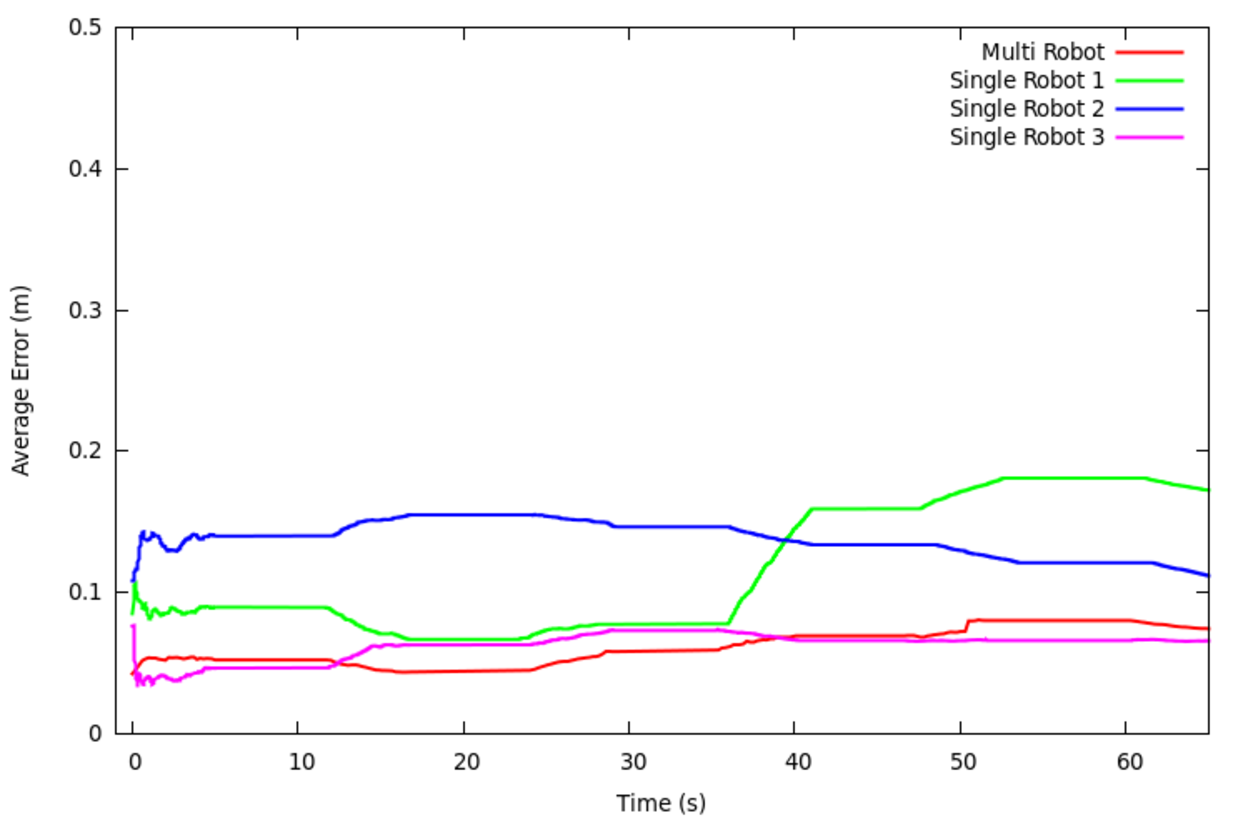
\includegraphics[width=0.8\linewidth]{Figures/Result-Scenario-3}
			};
		\end{tikzpicture}
	\end{figure}
\end{frame}
